\chapter{Prévisionnel du projet}
Maintenant que nous avons vu plusieurs solutions nous permettant de réaliser notre 
objectif, nous allons détailler les étapes qui seront réalisées pour la suite du projet.

\section{Outils utilisés}
Pour ce projet, nous devons utilisé la Kinect 2, ce qui impose certaines contraintes comme l'utilisation
du SDK de la caméra fourni par Microsoft.\\

Nous allons travailler sur l'environnement Unity3D qui est 
un environnement simple d'accès utilisant le langage C\#. Grâce à cette outils, nous pouvons
facilement importer un mesh de main, qui sera le modèle qui devra être utilisé pour modèliser
la main de l'utilisateur. Le fait que la plateforme utilise le langage C\# nous facilite 
l'accès au données fournies par la caméra.\\

Nous avons obtenu, de la part de l'équipe de recherche, une DLL comportant des fonctions permettant
de récupérer les coordonnées des articulations de la main de l'utilisateur. Cette DLL utilise 
la même méthode de reconnaissance des parties du corp \cite{export:145347}. Il reste à déterminer les 
étapes de réalisation du projet.

\section{Planification des tâches}
Nous avons décomposé le projet en plusieurs étapes afin d'avoir des objectifs réalisable en 
un minimum de temps avec certains objectif fesable en parallèle avec de pouvoir nous disperser
les tâches mieux. Le but étant de réaliser tout l'aspect recherche assez rapidement pour 
avoir plus de temps dans la réalisation d'une application démonstrative assez complète. Cette application
permettra de voir un maximum de fonctionnalité réalisable avec ce type d'interaction.\\

Nous allons dans un premier temps faire en sorte que nous puissions utiliser la DLL dans Unity3D.
Dans cette première étape il faut que nous récupérions les coordonnées des points des articulations
de la main de l'utilisateur. Pour nous allons appeler des fonctions présents dans la DLL dans un 
script C\# que nous placerons dans un objet vide d'une scène créée dans le moteur Unity3D.\\

Dans la seconde étape, nous devons modéliser les points des articulations de la main déterminer 
dans l'étape précédente. Il faut donc créé des objets dont les coordonnées seront ceux des articulations.
Pous cela il faudra passer par une phase de transformation des coordonées. En effet, les coordonnées
que nous récupérons via la DLL, ne seront pas forcément adapté à la scène créée dans Unity3D. Les 
objets qui représente les articulations de la main devront être créé dans le script afin qu'il 
soit visible seulement quand un utilisateur est détecté et qu'il puisse y avoir plusieurs main
détecté dans la même scène.\\

La troisième étape peut être réalisé indépendemment des deux première qui sont lié. Dans cette étape,
nous avons besoin de modéliser une main. Pour cela, nous avons besoin d'importer le mesh d'une main et
de réussir à modifier ce mesh dans le but de pour gérer le niveau de détail de la main. Cette dernière
partie est nécessaire pour que lors du mouvement de la main, il n'y est pas d'effet visuel indésirable.
Pour cela, il nous faudra utiliser la méthode décrite dans \cite{export:217428}.\\

La dernière étape est de faire correspondre les articulations de la main détecté dans l'étape deux avec
le mesh de la main. Cette méthode est expliqué dans \cite{export:217428}.

\begin{figure}
  \begin{center}
    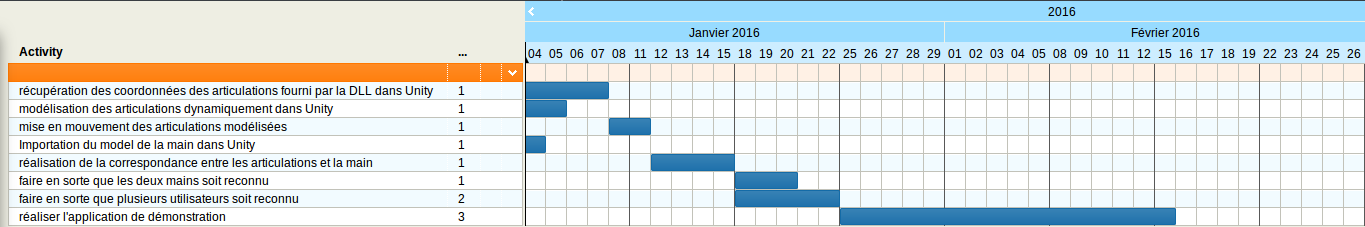
\includegraphics[angle=-90, width=4cm]{images/planning.png}
    \caption{Planning du projet}
    \label{fig:planning}
  \end{center}
\end{figure}
%TODO expliquer quel sera la demo de fin
